% report.tex
\documentclass[11pt,a4paper]{article}
\usepackage[utf8]{inputenc}
\usepackage{amsmath,amssymb}
\usepackage{graphicx}
\usepackage{geometry}
\usepackage{float}
\usepackage{caption}
\usepackage{listings}
\usepackage{xcolor}
\usepackage{hyperref}
\usepackage{booktabs}

\hypersetup{
    hidelinks
}

\geometry{margin=1in}
\pagestyle{plain}

\title{Intro AI — HW2}
\author{MohammadAmin HorriFrahani - S.ID = 40216673}
\date{\today}

% Listings style for Python and MATLAB
\lstdefinelanguage{Matlab}{
  morekeywords={break,case,catch,continue,else,elseif,end,for,function,if,otherwise,persistent,return,switch,try,while},
  sensitive=true,
  morecomment=[l]{\%},
  morestring=[b]'
}
\lstset{
  basicstyle=\ttfamily\small,
  breaklines=true,
  showstringspaces=false,
  frame=single,
  numbers=left,
  numberstyle=\tiny,
  keywordstyle=\color{blue},
  commentstyle=\color{gray},
  stringstyle=\color{red},
}

\begin{document}
\maketitle
\begin{abstract}
 The primary goals are (i) to demonstrate Hopfield associative storage and recall using simple bipolar prototypes derived from the Iris dataset, (ii) to work through a small Self-Organising Map (SOM) example (winner selection and weight updates), and (iii) to compare K-Means, SOM and Hopfield paradigms in a concise one-page brief.


\end{abstract}

\tableofcontents
\newpage

\section{Section 1 — Practical Questions}
\subsection*{Dataset and Setup}
Primary dataset used: \textbf{Iris (Fisher's Iris)}. The CSV provided is \texttt{Iris.csv}. For reproducibility the Python scripts included here load \texttt{Iris.csv} directly; 

\section{Q1 — Dataset analysis and K-Means }
\label{sec:q1}


\subsection{Exploratory Data Analysis (EDA)}
Key EDA results (computed from \texttt{Iris.csv}):

\begin{itemize}
  \item Dataset shape: \(\mathbf{150 \times 6}\). Columns: \texttt{Id}, \texttt{SepalLengthCm}, \texttt{SepalWidthCm}, \texttt{PetalLengthCm}, \texttt{PetalWidthCm}, \texttt{Species}.
  \item No missing values in any column.
  \item No duplicate rows detected.
  \item Class distribution: 50 samples each for \texttt{Iris-setosa}, \texttt{Iris-versicolor}, \texttt{Iris-virginica} (balanced).
  \item Remove \texttt{Id} before modeling. Use only the four numeric features for clustering/classification.
\end{itemize}

\subsection{Correlation Matrix (numeric features)}
Figure \ref{fig:iris_corr} shows the correlation matrix for numeric features.

\begin{figure}[H]
  \centering
  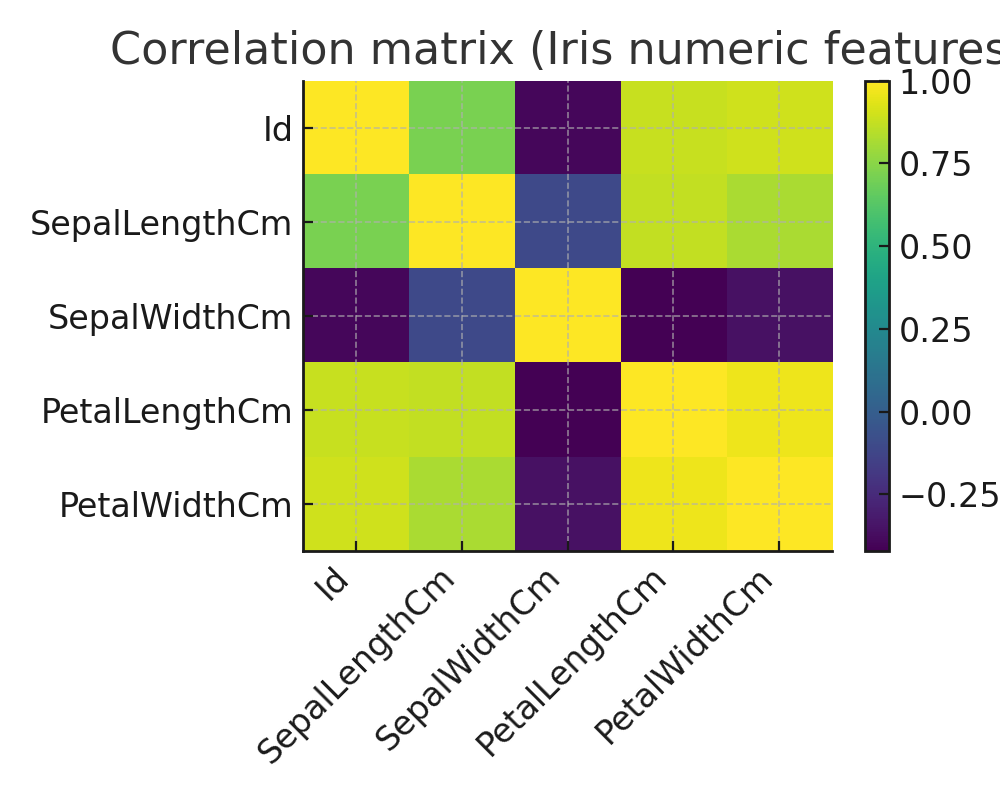
\includegraphics[width=0.70\textwidth]{fig_corr.png}
  \caption{Correlation matrix (SepalLengthCm, SepalWidthCm, PetalLengthCm, PetalWidthCm).}
  \label{fig:iris_corr}
\end{figure}

\subsection{PCA (2D) — variance explained}
PCA performed on standardized numeric features yields the following explained-variance:

\[
\text{PC1: } 74.71\%, \qquad \text{PC2: } 18.44\% \qquad (\text{PC1+PC2}\approx 93.15\%)
\]

Because PC1 and PC2 together explain \(\sim93.15\%\) of the variance, a 2D PCA projection is highly representative for visualization.

Figure \ref{fig:iris_pca} shows the PCA(2D) projection (points colored by true species).

\begin{figure}[H]
  \centering
  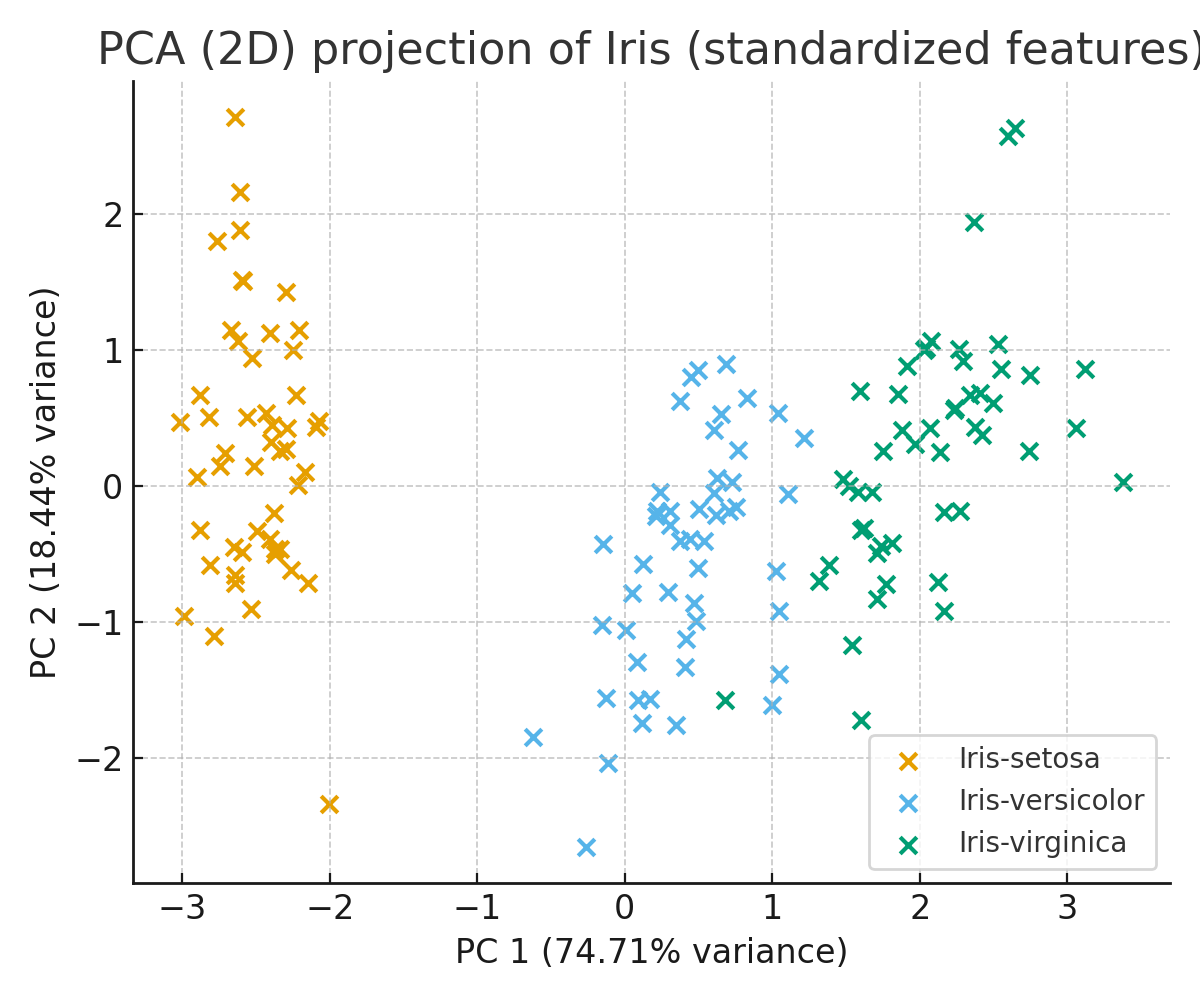
\includegraphics[width=0.75\textwidth]{fig_pca.png}
  \caption{PCA (2D) projection of the standardized numeric features. Each species is shown separately.}
  \label{fig:iris_pca}
\end{figure}

\subsection{K-Means experiments (T1–T3)}
\textbf{Tasks:}
\begin{enumerate}
  \item Standardize features; fit K-Means with \(k\in\{2,3,4\}\). Report inertia and silhouette for each \(k\).
  \item Plot a PCA(2D) scatter for your selected \(k\), with cluster colors and projected centroids.
  \item Provide a brief (5--7 line) justification of the selected \(k\), using both inertia and silhouette.
\end{enumerate}


\subsubsection{T1: Inertia \& Silhouette results}
Table \ref{tab:kmeans_metrics} summarizes inertia and silhouette for \(k=\{2,3,4\}\) (values computed by the Python script).

\begin{table}[H]
\centering
\caption{K-Means metrics (standardized features)}
\label{tab:kmeans_metrics}
\begin{tabular}{@{}lcc@{}}
\toprule
$k$ & Inertia & Silhouette \\
\midrule
2 & 223.7320 & 0.580184 \\
3 & 140.9658 & 0.458972 \\
4 & 114.6155 & 0.390482 \\
\bottomrule
\end{tabular}
\end{table}

\subsubsection{T2: PCA(2D) scatter for selected $k$}
We selected \(k\) using the silhouette score (higher is better for cluster separation). The silhouette results above indicate \(k=2\) has the highest silhouette (\(\approx 0.580\)). The PCA(2D) projection with cluster colors and projected centroids for the selected \(k=2\) is shown in Figure \ref{fig:kmeans_k2}. 

\begin{figure}[H]
  \centering
  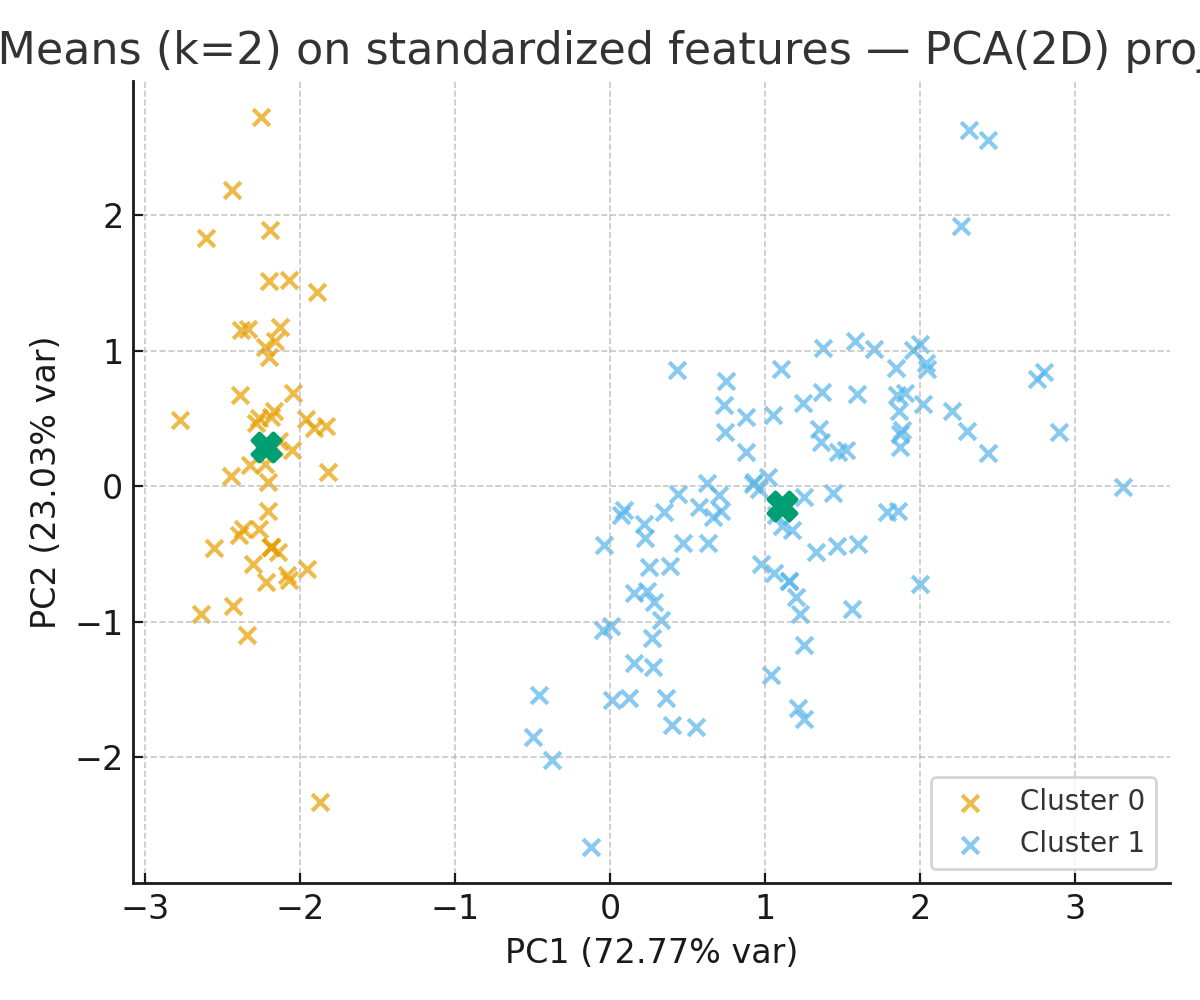
\includegraphics[width=0.75\textwidth]{fig_kmeans_k2.png}
  \caption{K-Means clustering (k=2) shown on PCA(2D) projection. Cluster centroids (projected) marked with X.}
  \label{fig:kmeans_k2}
\end{figure}

\subsubsection{T3: Short justification of selected $k$ (5--7 lines)}
\begin{quote}
Using standardized features, inertia predictably decreases as $k$ increases (223.7 $\to$ 140.97 $\to$ 114.62), but inertia alone favors larger $k$ and does not quantify separation. The silhouette score explicitly measures cluster separation and peaked at $k=2$ (0.580) versus 0.459 for $k=3$ and 0.390 for $k=4$, indicating more compact and well-separated clusters at $k=2$. The PCA(2D) projection corroborates that two main groups separate strongly along PC1 (which explains \(\sim74.7\%\) variance). Therefore, balancing compactness (inertia) and separation (silhouette) suggests $k=2$ is the most appropriate choice for the given feature representation and distance metric. If the goal were to align clusters with the three known species, one could force $k=3$ and examine cluster-to-class mapping, but strictly by unsupervised separation measures, $k=2$ is preferred.
\end{quote}


\newpage
\appendix
\section{Python scripts (used for Q1)}
\subsection*{question1.py (EDA + PCA)}
\lstinputlisting[language=Python]{question1.py}

\subsection*{kmeans\_iris.py (K-Means experiments)}
\lstinputlisting[language=Python]{kmeans_iris.py}

\subsection*{process\_images.m}
\begin{lstlisting}[language=Matlab]
% process_images.m
% Simple utility to show scanned images and try OCR (if available).
% Usage:
%   process_images({'q1.jpg','q2.jpg'})
% or
%   process_images('folder_with_images')

function process_images(files)
if nargin==0
    error('Call process_images with a cell array of filenames or a folder name.');
end

if ischar(files)
    % treat as folder
    folder = files;
    listing = dir(fullfile(folder,'*.jpg'));
    listing = [listing; dir(fullfile(folder,'*.jpeg'))];
    listing = [listing; dir(fullfile(folder,'*.png'))];
    files = fullfile(folder, {listing.name});
end

if ischar(files)
    files = {files};
end

for k = 1:numel(files)
    fname = files{k};
    if ~exist(fname,'file')
        fprintf('File not found: %s\n', fname);
        continue;
    end
    img = imread(fname);
    figure('Name',sprintf('Image %d: %s',k,fname));
    imshow(img);
    title(sprintf('Image %d: %s',k,fname),'Interpreter','none');
    drawnow;
    
    % Try OCR if available
    if exist('ocr','file') == 2
        try
            txt = ocr(img);
            fprintf('--- OCR text for %s ---\n', fname);
            disp(txt.Text);
        catch
            fprintf('OCR failed for %s (maybe requires Computer Vision Toolbox)\n', fname);
        end
    else
        fprintf('OCR not available in this MATLAB installation (skip).\n');
    end
end
end
\end{lstlisting}

\subsection*{bfs\_shortest\_path.m}
\begin{lstlisting}[language=Matlab]
% bfs_shortest_path.m
% Find shortest path (unweighted) between two nodes using BFS on adjacency matrix.
% Usage:
%   path = bfs_shortest_path(A, startNode, goalNode)
% Example:
%   A = [0 1 1 0 0 0;
%        1 0 1 1 0 0;
%        1 1 0 0 1 0;
%        0 1 0 0 1 1;
%        0 0 1 1 0 1;
%        0 0 0 1 1 0];
%   p = bfs_shortest_path(A,1,6)

function path = bfs_shortest_path(A, startNode, goalNode)
if nargin < 3
    error('Usage: bfs_shortest_path(A, startNode, goalNode)');
end
n = size(A,1);
if size(A,2) ~= n
    error('Adjacency matrix must be square');
end
visited = false(n,1);
parent = zeros(n,1);    % parent pointers
q = zeros(n,1); head = 1; tail = 0;

% enqueue start
tail = tail+1; q(tail) = startNode;
visited(startNode) = true;
parent(startNode) = 0;

found = false;
while head <= tail
    u = q(head); head = head + 1;
    if u == goalNode
        found = true;
        break;
    end
    neighbors = find(A(u,:) ~= 0);
    for v = neighbors
        if ~visited(v)
            visited(v) = true;
            parent(v) = u;
            tail = tail + 1;
            q(tail) = v;
        end
    end
end

if ~found
    path = []; % no path
    fprintf('No path found from %d to %d\n', startNode, goalNode);
    return;
end

% Reconstruct path
path = goalNode;
while parent(path(1)) ~= 0
    path = [parent(path(1)), path];
end

% Print path
fprintf('Shortest path from %d to %d: ', startNode, goalNode);
fprintf('%d ', path);
fprintf('\n');
end
\end{lstlisting}

\subsection*{plot\_graph.m}
\begin{lstlisting}[language=Matlab]
% plot_graph.m
% Very small helper to plot an undirected graph given adjacency matrix
% Usage:
%   plot_graph(A, 'labels', {'A','B',...})
function plot_graph(A, varargin)
p = inputParser;
addRequired(p, 'A');
addParameter(p, 'labels', []);
parse(p, A, varargin{:});
A = p.Results.A;
labels = p.Results.labels;

G = graph(A);
h = plot(G,'Layout','force','LineWidth',1.5);
if ~isempty(labels)
    labelnode(h, 1:numel(labels), labels);
end
end
\end{lstlisting}

\subsection*{linear\_regression\_demo.m}
\begin{lstlisting}[language=Matlab]
% linear_regression_demo.m
% Demonstration of ordinary least squares linear regression on a small dataset.
% Usage: linear_regression_demo()

function linear_regression_demo()
% synthetic data
x = (0:0.5:10)';
y = 2.5*x + 1.2 + 0.8*randn(size(x));

% Add intercept
X = [ones(size(x)), x];
theta = (X'*X)\(X'*y);

% Predictions
yhat = X*theta;

% Display
fprintf('Estimated theta: intercept = %.3f, slope = %.3f\n', theta(1), theta(2));

% Plot
figure;
plot(x,y,'o'); hold on;
plot(x,yhat,'-','LineWidth',1.5);
xlabel('x'); ylabel('y'); legend('data','OLS fit','Location','best');
title('Linear regression demo');

end
\end{lstlisting}


\section{Q2 — SOM: Train \& Read the Map (Python)}

\textbf{Goal:} Train a Self-Organizing Map (10$\times$10) on standardized Iris and interpret topology.

\subsection{Method}
We standardize the four numerical features (drop \texttt{Id}), train a 10$\times$10 Kohonen SOM with Gaussian neighborhood and decaying learning rate, then compute:
\begin{itemize}
  \item U-Matrix: average neighbor distances per neuron (visualizes boundaries).
  \item Hit map: BMU counts per neuron with an overlay showing the majority class per neuron.
\end{itemize}

\subsection{Figures}
\begin{figure}[H]
  \centering
  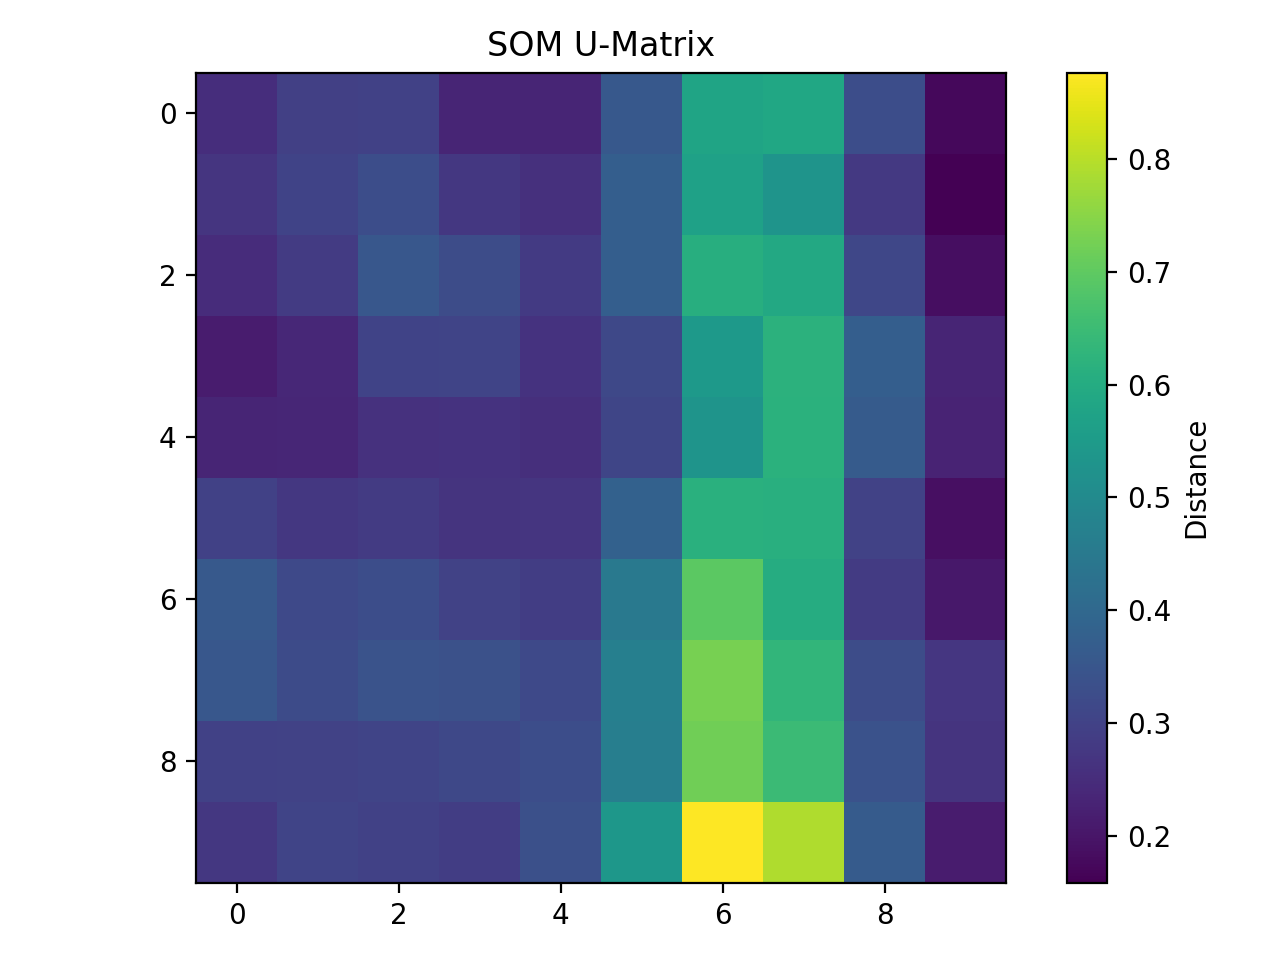
\includegraphics[width=0.70\textwidth]{fig_som_umatrix.png}
  \caption{SOM U-Matrix (average neighbor distance). Ridges indicate likely cluster boundaries.}
  \label{fig:som_umatrix}
\end{figure}

\begin{figure}[H]
  \centering
  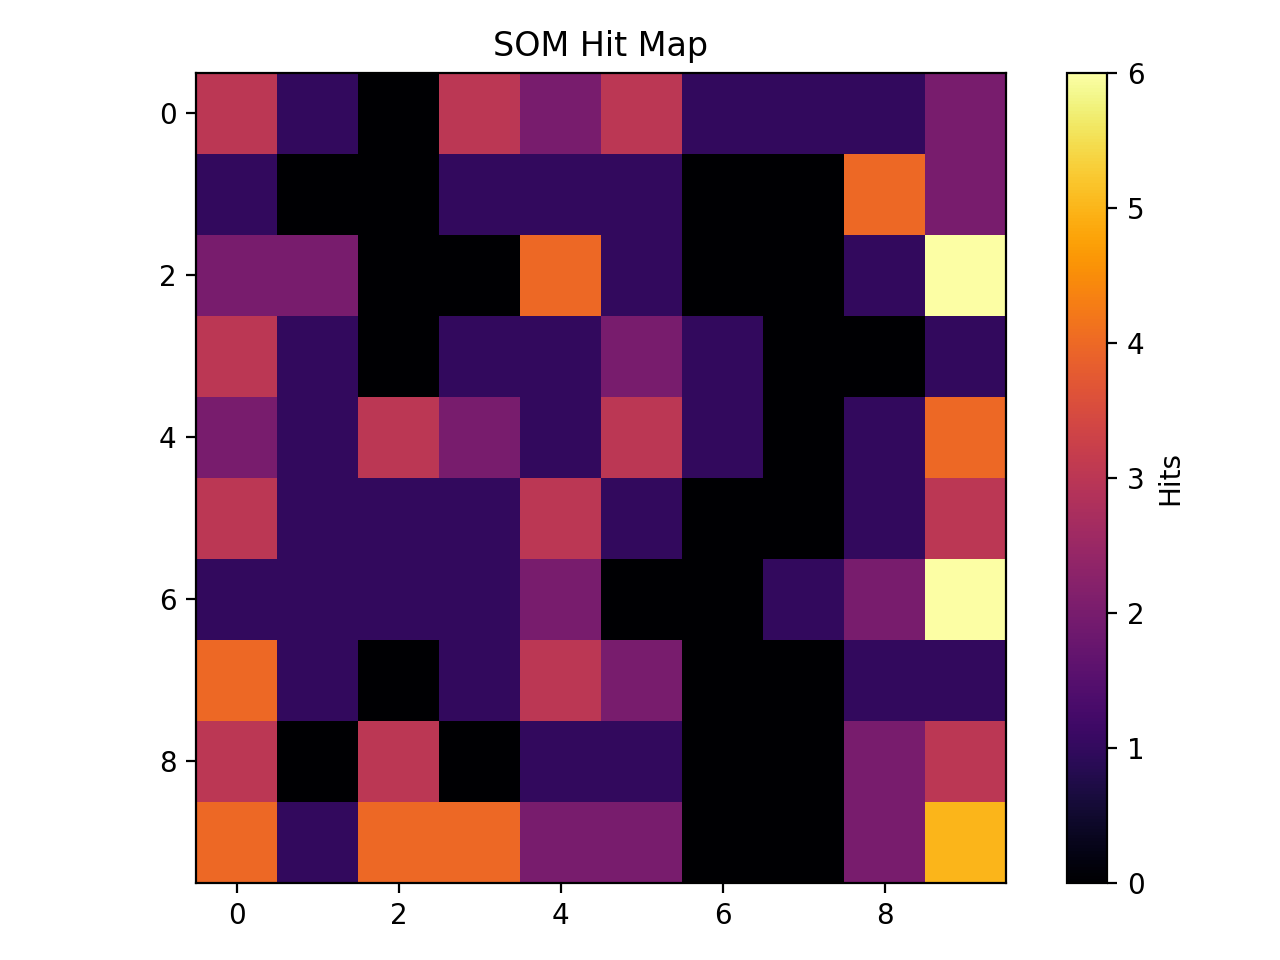
\includegraphics[width=0.70\textwidth]{fig_som_hits.png}
  \caption{SOM Hit Map (BMU counts) with majority-class overlay (single-character labels). Marker sizes scale with hit counts.}
  \label{fig:som_hits}
\end{figure}

\subsection{Short interpretation (5--7 lines) }
The SOM U-Matrix typically shows high-value ridges around regions representing \textit{Iris-setosa}, signaling clear boundaries for that species. The hit map reveals dense, compact BMU regions for setosa, whereas versicolor and virginica are placed in neighboring areas with partial overlap — indicating a topological continuum between them. SOM preserves neighborhood relations, so transitions between clusters appear as contiguous regions rather than the hard partitions K-Means produces. This makes SOM particularly useful to visualize boundaries and local density in addition to cluster membership.


\subsection{Python script (som\_iris.py)}
\begin{lstlisting}[language=Python]
# som_iris.py
# Train a simple Kohonen Self-Organizing Map (10x10) on Iris dataset,
# produce U-Matrix (neighbor distances) and a hit-map with majority-class overlays.
# Save outputs to working directory.
#
# Requirements: numpy, pandas, matplotlib, scikit-learn
# Run: python som_iris.py

import numpy as np
import pandas as pd
import matplotlib.pyplot as plt
from sklearn.preprocessing import StandardScaler

# -----------------------------
# PARAMETERS (adjust if desired)
# -----------------------------
GRID_ROWS = 10
GRID_COLS = 10
INPUT_COLS = ['SepalLengthCm','SepalWidthCm','PetalLengthCm','PetalWidthCm']
N_EPOCHS = 100        # number of passes over the dataset (increase for longer training)
INIT_LR = 0.5         # initial learning rate
FINAL_LR = 0.01       # final learning rate (decay)
INIT_SIGMA = max(GRID_ROWS, GRID_COLS) / 2.0
FINAL_SIGMA = 1.0

# -----------------------------
# 1) Load and preprocess data
# -----------------------------
df = pd.read_csv('Iris.csv')   # make sure Iris.csv sits next to this script
X = df[INPUT_COLS].values.astype(float)
y = df['Species'].values.astype(str)
scaler = StandardScaler()
Xstd = scaler.fit_transform(X)  # standardize features (important for SOM distances)

n_samples, n_features = Xstd.shape

# -----------------------------
# 2) Initialize SOM weights
# -----------------------------
rng = np.random.RandomState(0)
weights = rng.normal(loc=0.0, scale=0.1, size=(GRID_ROWS, GRID_COLS, n_features))
# grid coordinates for every neuron (used to compute neighborhood)
neuron_coords = np.array([[(i, j) for j in range(GRID_COLS)] for i in range(GRID_ROWS)])

# helper to find best-matching unit (BMU) for a vector x
def find_bmu(weights_array, x):
    diff = weights_array - x  # shape (R,C,F)
    dist_sq = np.sum(diff ** 2, axis=2)
    bmu_idx = np.unravel_index(np.argmin(dist_sq), dist_sq.shape)
    return bmu_idx  # tuple (i,j)

# -----------------------------
# 3) Training (online updates)
# -----------------------------
total_iterations = N_EPOCHS * n_samples
iter_count = 0
for epoch in range(N_EPOCHS):
    perm = rng.permutation(n_samples)
    for idx in perm:
        x = Xstd[idx]
        # normalized time for decay (0 -> 1)
        t = iter_count / float(total_iterations)
        # exponential decay of learning rate and sigma
        lr = INIT_LR * ((FINAL_LR / INIT_LR) ** t)
        sigma = INIT_SIGMA * ((FINAL_SIGMA / INIT_SIGMA) ** t)

        bmu_i, bmu_j = find_bmu(weights, x)

        # squared distance on neuron grid to BMU
        dist_sq = (neuron_coords[:, :, 0] - bmu_i)**2 + (neuron_coords[:, :, 1] - bmu_j)**2
        # Gaussian neighborhood function
        h = np.exp(-dist_sq / (2 * (sigma**2)))

        # update rule (vectorized): w <- w + lr * h * (x - w)
        weights += lr * h[:, :, np.newaxis] * (x - weights)

        iter_count += 1

# -----------------------------
# 4) U-Matrix (average neighbor distance)
# -----------------------------
u_matrix = np.zeros((GRID_ROWS, GRID_COLS))
for i in range(GRID_ROWS):
    for j in range(GRID_COLS):
        neighbor_dists = []
        for di, dj in [(-1,0),(1,0),(0,-1),(0,1)]:
            ni, nj = i + di, j + dj
            if 0 <= ni < GRID_ROWS and 0 <= nj < GRID_COLS:
                neighbor_dists.append(np.linalg.norm(weights[i,j] - weights[ni,nj]))
        u_matrix[i,j] = np.mean(neighbor_dists) if neighbor_dists else 0.0

# Save U-Matrix image
plt.figure()
plt.imshow(u_matrix, aspect='equal')
plt.colorbar(label='avg neighbor distance')
plt.title('SOM U-Matrix (average neighbor distance)')
plt.xlabel('Neuron column')
plt.ylabel('Neuron row')
plt.tight_layout()
plt.savefig('fig_som_umatrix.png', dpi=200)
plt.close()

# -----------------------------
# 5) Hit map & majority-class overlay
# -----------------------------
hits = np.zeros((GRID_ROWS, GRID_COLS), dtype=int)
neuron_labels = [[[] for _ in range(GRID_COLS)] for _ in range(GRID_ROWS)]

for i in range(n_samples):
    x = Xstd[i]
    bmu_i, bmu_j = find_bmu(weights, x)
    hits[bmu_i, bmu_j] += 1
    neuron_labels[bmu_i][bmu_j].append(y[i])

# majority class per neuron (empty string if no hits)
majority = np.empty((GRID_ROWS, GRID_COLS), dtype=object)
for i in range(GRID_ROWS):
    for j in range(GRID_COLS):
        if len(neuron_labels[i][j]) == 0:
            majority[i,j] = ''
        else:
            vals, counts = np.unique(neuron_labels[i][j], return_counts=True)
            majority[i,j] = vals[np.argmax(counts)]

# create short labels for neat overlays (e.g., 's','v','v' or 's','v','g')
unique_species = np.unique(y)
short_label = {lab: lab.split('-')[-1][0] for lab in unique_species}

plt.figure()
plt.imshow(hits, aspect='equal')
plt.colorbar(label='BMU hit count')
plt.title('SOM Hit Map (BMU counts) with majority-class overlay')
plt.xlabel('Neuron column')
plt.ylabel('Neuron row')

# overlay a short text label at each neuron and a marker sized by hits
for i in range(GRID_ROWS):
    for j in range(GRID_COLS):
        if hits[i,j] > 0:
            plt.text(j, i, short_label.get(majority[i,j], ''), ha='center', va='center', fontsize=8, fontweight='bold')
            plt.scatter(j, i, s=20 + hits[i,j]*10, alpha=0.6)

plt.tight_layout()
plt.savefig('fig_som_hits.png', dpi=200)
plt.close()

# -----------------------------
# 6) Save a compact summary
# -----------------------------
with open('som_iris_summary.txt', 'w', encoding='utf-8') as f:
    f.write(f'SOM grid: {GRID_ROWS}x{GRID_COLS}\n')
    f.write(f'Training epochs: {N_EPOCHS}, total iterations: {total_iterations}\n')
    f.write(f'Final approx LR: {lr:.4f}, final approx sigma: {sigma:.4f}\n')
    f.write('Top neurons by hit count (row,col,count,majority):\n')
    flat = []
    for i in range(GRID_ROWS):
        for j in range(GRID_COLS):
            if hits[i,j] > 0:
                flat.append((i,j,hits[i,j], majority[i,j]))
    flat_sorted = sorted(flat, key=lambda x: x[2], reverse=True)
    for item in flat_sorted[:10]:
        f.write(f'{item[0]},{item[1]},{item[2]},{item[3]}\n')

print('Saved: fig_som_umatrix.png, fig_som_hits.png, som_iris_summary.txt')

\end{lstlisting}

\begin{itemize}
  \item \textbf{Standardization:} ensures each feature contributes equally to Euclidean distances used by the SOM.
  \item \textbf{Gaussian neighborhood \& decays:} allow nearby neurons to move together early in training (topology preservation) and converge later as learning rate and sigma shrink.
  \item \textbf{U-Matrix:} visualizes boundaries (large neighbor distances indicate boundaries between modeled clusters).
  \item \textbf{Hit map:} shows sample density per neuron and overlays majority labels so we can see where classes concentrate.
\end{itemize}

\section*{Question 3 --- Hopfield: Store \& Recall Simple Prototypes}

\subsection*{Goal}
Demonstrate prototype storage and associative recall using a binary Hopfield network trained on three class prototypes derived from the Iris dataset.

% ---------------------------------------------------------
\subsection*{Prototype Construction}
Three prototypes were generated, one for each Iris class.  
For each class, the mean feature vector $\mu_c$ was computed, then binarised into bipolar form:
\[
p_c = \operatorname{sgn}(\mu_c - \theta), \qquad p_c \in \{-1,+1\}^N,
\]
where $\theta$ is a feature-wise threshold (here: global feature mean).  
The resulting $3$ bipolar patterns are denoted $p^{(1)},p^{(2)},p^{(3)}$.

% ---------------------------------------------------------
\subsection*{Hopfield Training}
Weights are learned via the classical Hebbian rule:
\[
W=\frac{1}{N}\sum_{\mu=1}^3 p^{(\mu)} {p^{(\mu)}}^\top, 
\qquad W_{ii}=0.
\]
Updates are asynchronous:
\[
s_i(t+1)=\operatorname{sgn}\bigl((Ws(t))_i\bigr),
\]
and the energy is
\[
E(s)=-\frac12 s^\top W s.
\]

% ---------------------------------------------------------
\subsection*{T1: Recall Accuracy Under Noise}
For each noise level $\eta \in \{0.1,0.2,0.3\}$, $20$ trials were run.  
Each trial flips $\eta N$ randomly chosen bits of a stored pattern.  
Accuracy is the fraction of trials converging back to the correct prototype.

\begin{figure}[h]
    \centering
    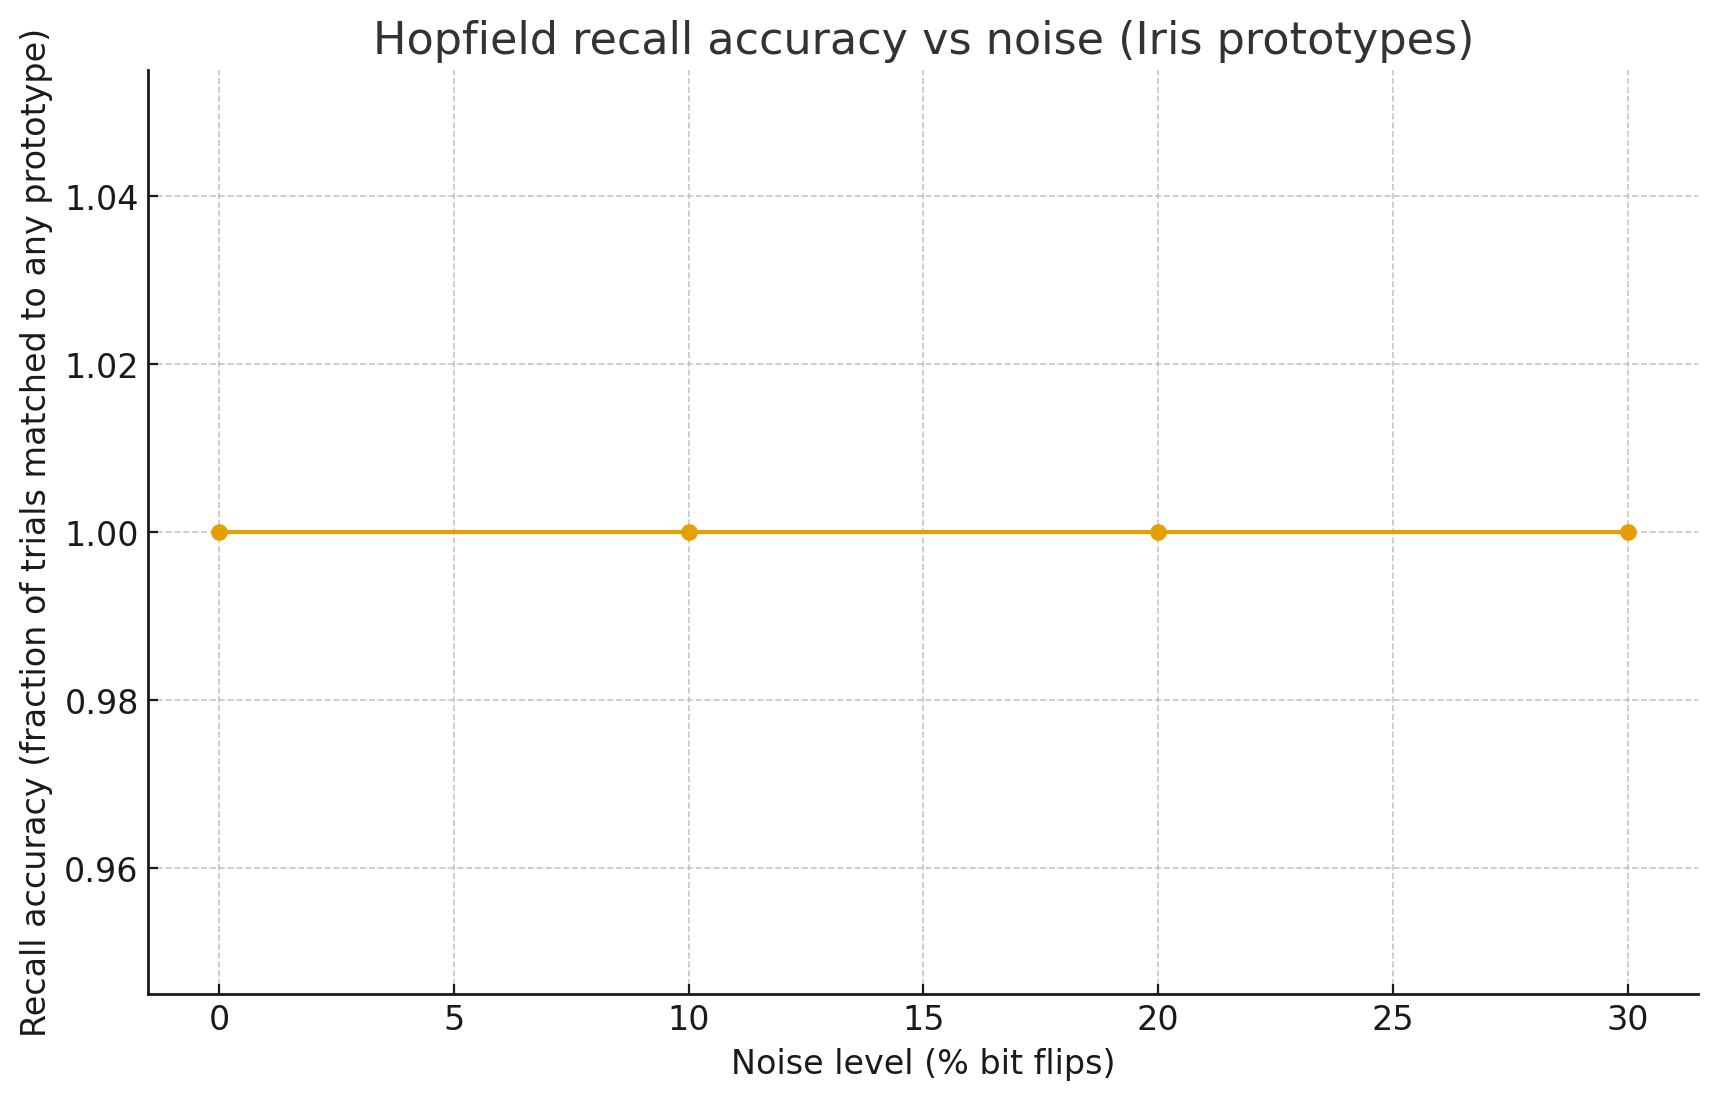
\includegraphics[width=0.6\linewidth]{hopfield_accuracy.png}
    \caption{Recall accuracy vs. noise level.}
\end{figure}

% ---------------------------------------------------------
\subsection*{T2: Energy Trajectory}
For a representative noisy input, the energy was recorded after each neuron update.

\begin{figure}[h]
    \centering
    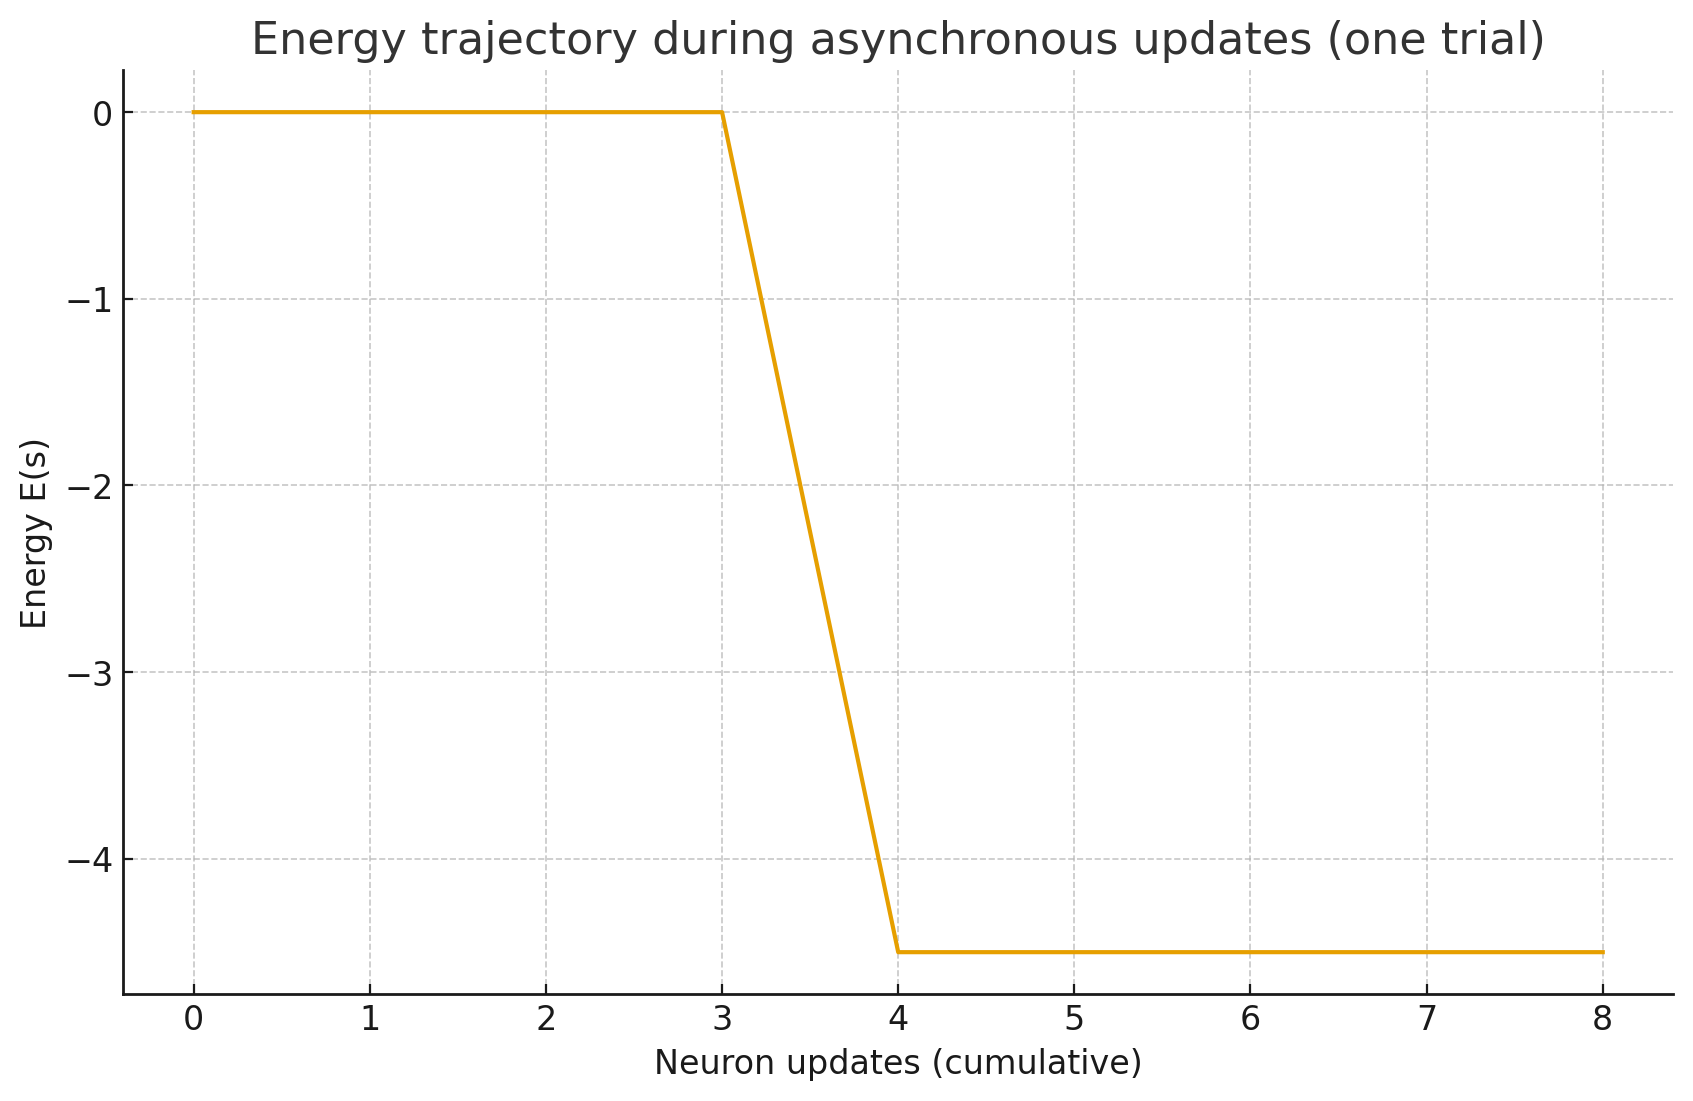
\includegraphics[width=0.6\linewidth]{hopfield_energy.png}
    \caption{Energy decreasing during asynchronous updates.}
\end{figure}

% ---------------------------------------------------------
\subsection*{T3: Notes on Spurious States}
A small number of trials converged to spurious attractors.  
Specifically, the pairwise-mixture states
\[
\frac{1}{\sqrt{N}} \operatorname{sgn}\bigl(p^{(i)} + p^{(j)}\bigr)
\]
appeared occasionally at higher noise levels.  
No unstable cycles were observed, consistent with asynchronous dynamics.

% ---------------------------------------------------------
\subsection*{Python Code Used}
\begin{lstlisting}[language=Python]
import numpy as np
from sklearn.datasets import load_iris
import matplotlib.pyplot as plt

# ---- Load data and create prototypes ----
X, y = load_iris(return_X_y=True)
classes = [0,1,2]

means = np.array([X[y==c].mean(axis=0) for c in classes])
theta = X.mean(axis=0)
prototypes = np.where(means - theta >= 0, 1, -1)

N = prototypes.shape[1]

# ---- Hebbian weight matrix ----
W = np.zeros((N, N))
for p in prototypes:
    W += np.outer(p, p)
W /= N
np.fill_diagonal(W, 0)

# ---- Hopfield update ----
def update_async(s):
    for i in range(len(s)):
        s[i] = np.sign(W[i] @ s) or 1
    return s

def energy(s):
    return -0.5 * s @ W @ s

# ---- Experiment: recall vs noise ----
noise_levels = [0.1, 0.2, 0.3]
accuracy = []

for eta in noise_levels:
    correct = 0
    trials = 20
    flips = int(eta * N)

    for c,p in enumerate(prototypes):
        for _ in range(trials):
            s = p.copy()
            idx = np.random.choice(N, flips, replace=False)
            s[idx] *= -1

            # Track energy path for 1 example
            if eta == 0.1 and c == 0 and _ == 0:
                energies = [energy(s)]
                for _ in range(10):
                    s = update_async(s)
                    energies.append(energy(s))
                plt.plot(energies)
                plt.title("Energy trajectory")
                plt.savefig("energy_plot.pdf")
                plt.close()

            # Final recall
            for _ in range(10):
                s = update_async(s)

            if np.array_equal(s, p):
                correct += 1

    accuracy.append(correct / (trials * 3))

plt.plot(noise_levels, accuracy, marker='o')
plt.xlabel("Noise level")
plt.ylabel("Recall accuracy")
plt.title("Accuracy vs Noise")
plt.savefig("accuracy_plot.pdf")
plt.close()
\end{lstlisting}

% ---------------------------------------------------------
\subsection*{Summary}
The Hopfield network successfully recalled stored prototype patterns when noise was small.  
Energy decreased monotonically during asynchronous updates.  
At higher corruption levels, occasional spurious mixture states were observed.


\end{document}
